% Chapter Template
\part{Physics introduction}
\chapter{The Standard Model and Beyond} \label{Chapter1} 

\section{Introduction}
Starting from late 19th century and progressing in the first half of the 20th century, 
the theories and discoveries of thousands of physicists have led to a significant insight into the fundamental structure of matter. 
By the 1960s, physicists had promote quite a collection of what they assumed to be fundamental particles, basic building blocks of matter that could not be resolved any further into sub-pieces. 

In 1964, theorists Murray Gell-Mann~\cite{GELLMANN1964214} and George Zweig~\cite{Zweig:570209} theorized that many components of the so-called ``particle zoo'' were composite particles consisted of even smaller parts, which are now called quarks. The list of fundamental particles was further reduced, the description of the fundamental forces which govern the interaction between them was added and new patterns were begun to appear. This was the outset of the development of the Standard Model of particle physics.
The first references to the so-called “standard model” can be found in papers published in the 1970s~\cite{Pais:1975gn,PhysRevD.13.680} and only in the '80s and '90s the \emph{S} and \emph{M} got capitalized.

To this day, the Standard Model (SM) has successfully interpreted nearly all experimental results and accurately predicted a wide variety of phenomena getting even more credits with the latest foreseen discoveries such as top quark observation (1995) and Higgs boson discovery (2012). Even though it is considered the most solid description of the subatomic world, we see some holes when trying to address the full picture.\\
Those unexplained aspects, which are going to be specified in Sec.~\ref{sec:bsm}, have inspired the big hunt for new physics that has drawn the creation of so many new experiments and that has fed fresh exotic theories. This thesis cooperates in this attempt.


\section{The Standard Model of Elementary Particles}
Figure~\ref{fig:SMfig} shows the building blocks of the Standard Model, either they are matter particles, everyday matter
or exotic matter created in particle accelerators and in the early universe, or they are the additional force-carrier particles.

In the Standard Model, the elementary particles are grouped into two main categories on the basis of the statistic they obey and consequently of the spin: fermions and bosons. 
\begin{figure}[h]
\centering
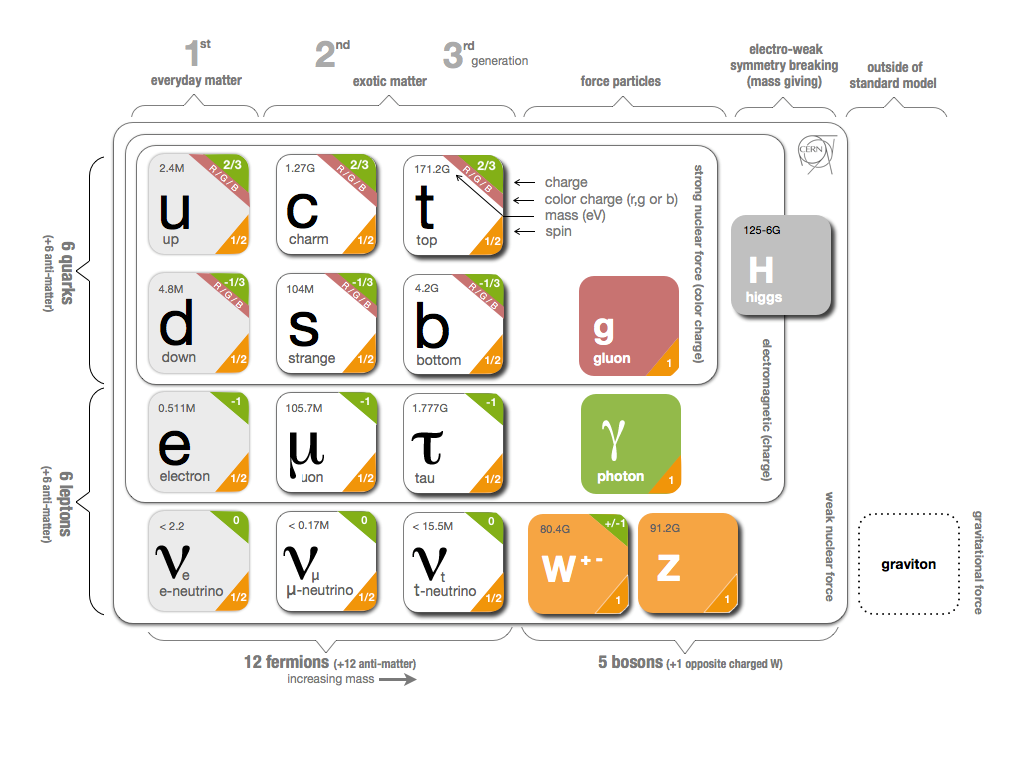
\includegraphics[clip,trim=1cm 2cm 2cm 1cm, width=0.75\textwidth]{Figures/c1/SMinfographic_image.png}
\caption{Elementary particles of the Standard Model (infographic
  developed for~\cite{particlefest})}
\label{fig:SMfig}
\end{figure}

The fermions are particles which follow the Fermi-Dirac statistic and correspondingly have half odd integer spin (1/2, 3/2, 5/2...). They do obey the Pauli exclusion principle and therefore they have different symmetry properties, with respect to bosons, when exchanging of two identical particles: the total wave function of a system of two identical fermions is antisymmetric for fermions. This lead to the fact that, in a rigorous way, if two identical (in spin and space coordinates) fermions interchange the total wave function changes its sign. Thus, two or more identical fermions can not simultaneously exist in the same quantum state. On the contrary particles with an integer spin like the bosons which follow the Bose-Einstein statistic do not obey the Pauli exclusion principle and can occupy the same quantum state. 

In the Standard Model, there are two types of elementary fermions: quarks (which form hadrons such as protons and neutrons) and leptons. 
Moreover, the fermions are grouped in three generations and each generation has two types of leptons and two quarks. The two leptons have one electric charge -1, the other one is neutral; the two quarks have charges $-1/3$ (down-type) and $+2/3$ (up-type). Between generations electric and strong interactions are identical while particles differ by their flavor quantum number and mass.  The first generation consists of electrons ($e$) and electron neutrinos ($\nu_e$) and of quarks \emph{up} and \emph{down}. All the everyday matter is composed by up-down quarks and electrons. The second generation is made of muons ($\mu$) and muon neutrinos ($\nu_\mu$) and of quarks \emph{charm} and \emph{strange}. The third generation is composed by taus ($\tau$) and tau neutrino ($\nu_\tau$) and by quarks \emph{top} and \emph{bottom}. The particles of higher generation have larger masses than the preceding one, this has the effect that leptons and quarks of the second and third families are more unstable with shorter life-time and can easily decay back to elements from the first generation.\\
Each of the 12 fermions has an anti-matter particle which presents all the charges reversed.

The fermions, just described, interact exchanging the bosons particles. The elementary bosons are force carriers and each of them is associated to a fundamental force. The photon ($\gamma$) is the mediator of the electromagnetic force, it has spin equal to 1, it is neutral and massless. The $\PW^{\pm}$ and \PZ are mediators of the weak force, they have spin 1, the $\PW^{\pm}$ have unitary charge (+1 or -1) while \PZ is neutral; the are heavy in mass ($M_\PW =\:$80.379 $\pm$ 0.012\GeV~\cite{pdgw}, $M_\PZ =\:$91.1876 $\pm$ 0.0021\GeV~\cite{pdgz}) and very short-lived. The quarks possess color charge which means they are subject to the strong interaction mediated by the gluons ($g$) which likewise are associated to a color charge. For a property of the strong interaction known as color confinement, quarks can not exist isolated. Thereupon quarks and gluons must cluster together to for hadrons which are color neutral (white) and which can exist and propagate freely. The hadrons can be made of either a quark and anti-quark, \emph{mesons} or three quarks, \emph{baryons}. The mesons are composite bosons (spin 0 or 1) while baryons are composite fermions. Quarks, besides interacting through strong force, could also transform into quarks of another flavor through weak interaction by absorbing/emitting a \PW boson. The strenghts/probabilities of the weak interactions between the six quarks do not have all the same magnitude (some are more preferable) and they are described by the values in the Cabibbo–Kobayashi–Maskawa matrix~\cite{10.1143/PTP.28.870}.\\
The massive bosons get their mass thanks to the interaction with the quantum field. The so-called Brout–Englert–Higgs (BEH) mechanism refers to the generation of masses for the three weak gauge bosons (\PW, \PZ) through electroweak symmetry breaking~\cite{PhysRevLett.13.321,PhysRevLett.13.508}. The mathematical treatment of Standard Model and of the BEH mechanism is presented in Sec.\ref{sec:mathSM}.\\
The last fundamental force, gravity, is not included in the Standard Model framework. 

The leptons are not affected by the strong interaction while they are subject to electromagnetic and weak interactions. As already said, the six leptons are organized in three generations, then are arranged in three left-handed weak isospin doublets where charged and neutral leptons share the same left-handed helicity. Each doublet has a different lepton number which has to be conserved during all the interactions implying that leptons and anti-leptons must be created in pairs of a single generation. The only violation of this universal lepton number conservation can be observed in weak interaction in the neutrino oscillations where is there a transformation between different generations. The neutrino oscillation and the obvious consequences are going to be extensively explained in Sec.~\ref{sec:bsm}. 


\section{The mathematical framework of the Standard Model}\label{sec:mathSM}


%-----------------------------------
%	SECTION 2
%-----------------------------------
\section{Beyond the Standard Model}\label{sec:bsm}
